% vim:ts=4:sw=4
% Copyright (c) 2014 Casper Ti. Vector
% Public domain.

\chapter{基于贪心的高速公路关键路段识别模型}
		本章主要分四个部分。第一节讲述了关键路段挖掘的意义,分析了现有研究的不足;第二节定义了高速公路关键路段挖掘模型,并给出次模性证明;第三节针对不同的挖掘方法进行实验,从多个角度分析本文方法的效果;第四节对本章内容做了一个小结。
		\section{引言}
		对于交通运输\parencite{NewmanBasic}、水利传输\parencite{test}、能源和通信等基础设施系统,在遭遇自然灾害或者人为灾害时,会对整个系统的性能造成显著的影响,带来重大的经济损失。所以在发生事故或者自然灾害的时候,维护这些网络的完整性至关重要。

		灾难管理是一个多阶段的过程,从防灾减灾和准备,着眼于长期消除或降低风险的措施,延伸到灾后 响应、恢复与重构。投资 基础设施系统在缓解中起着至关重要的作用 活动,它可以增强链接的稳定性。但是,将所有的路段稳定性都增强到坚不可摧,在管理人员看来是十分浪费的。本章节主要研究如何在有限的资源下,找到可以最大化网络通行效率的关键路段集合。将资源布置到这个关键路段集合中,最大化提升关键路段通行效率,增加路网稳定性,实现事故前的预防,事故后的快速恢复。

		本章主要研究如何对高速公路关键路段挖掘问题进行建模,并且围绕安徽、山西、北京的收费站车辆数据,进行真实数据集上的实验。

		\section{问题定义}
			\subsection{问题定义}
			高速公路具有成网性,给定一个有向图$G=\{V,E\}$,其中V代表收费站(节点)的集合;E表示高速公路中路段的集合。对于经过高速公路的车辆,定义O为车辆的出发节点,D作为车辆的目标节点。定义$P_e$($0\leqslant P_e\leqslant 1$)为路段的损毁率,这个概率通过历史上的高速公路路段损毁事件得到,同时可以随着交通管理者对路段进行管理而减小。定义管理者的决策向量y=\{$y_1$,$y_2$,$\cdots$,$y_n$\},y是一个n维向量,每一维$y_i$的数值取0或1,1表示这条路段属于关键路段集合,管理者会对其进行维护和投资管理,改善路段状况;0表示非关键路段。基于每一条路段都有一定概率损毁,定义$C_{e_i}$表示第i个路段的状态。当$C_{e_i}$等于1时,路段保持完好,当$C_{e_i}$等于0时,路段因为事故损毁。定义$\bm{c}$=\{$C_{e_1}$,$C_{e_2}$,$\cdots$,$C_{e_n}$\},c表示路网的某一种拓扑结构,$\bm{C}$表示路网的所有拓扑结构的集合。对于行驶在高速公路上的车辆,定义车辆的出行时间为$X_i$,这个出行时间由车辆的路径选择、出行时途径路径的车流密度决定。定义当高速公路路段断裂严重,车辆无法抵达目的地时,车辆的出行时间定为常量M。M的大小在一定程度上代表了路网连通性的权重,M越大,高速网络的连通性就越重要。为了更好的求解目标函数,在此提出两个假设:

			1)路段之间的损毁概率相互独立:假设处于静态模型下,所有路段都有一定的概率损毁,这些损毁率之间没有相互影响。传统研究网络可靠性的相关文献[3]都是基于这个假设所做的研究。

			2)M>Max($X_i$):M必须要大于连通路网中的最大出行代价。当车辆在路段中找不到一条可以抵达终点的路径时,定义车辆此次出行的代价要绝对大于路段仍然连通情况下的任意时间。即默认断裂对路网造成的影响大于路段仍然连通的情况。

			根据高速公路的历史事故数据,通过结构分析和统计调查[23],确定路段损毁的概率。使用该概率作为本研究的先验概率。高速公路建设管理者可以通过在高速路段上建立基础设施,投放人力资源等方式管理路段,增强路段的稳定性。假设路段$e$以概率$P_e$损毁,以概率$(1-P_e)$保持完好。基于路段的损毁率,我们可以计算路网拓扑结构概率矩阵Z:

		\[\begin{array}{*{20}{c}}
		{C_{{e_1}}^1}&{C_{{e_2}}^1}& \cdots &{C_{{e_n}}^1}&{{P^1}}\\
		{C_{{e_1}}^2}&{C_{{e_2}}^2}& \cdots &{C_{{e_n}}^2}&{{P^2}}\\
		 \vdots & \vdots & \ddots & \vdots & \vdots \\
		{C_{{e_1}}^m}&{C_{{e_2}}^m}& \cdots &{C_{{e_n}}^m}&{{P^m}}
		\end{array}\]
		矩阵中,$C_{{e_i}}$表示第i条路段的状态,0表示遭遇事故,已经损毁,1表示完好无损;对于每一行来说,前n项$C^j = \{{C_{{e_1}}^j},{C_{{e_2}}^j},\cdots,{C_{{e_n}}^j}\}$表示路网的拓扑结构,全0表示全部路段断裂,路网瘫痪;全1表示路网完全连通。第n+1项$P^j$表示高速公路网络拓扑变成这个拓扑结构的概率。其中$P^j \ = \ \prod\limits_{i = 1}^n {({P_{{e_i}}}C_{{e_i}}^j + (1 - {P_{{e_i}}})} (1 - C_{{e_i}}^j))$。在交通管理者选取关键路段,并进行一定的决策处理后,路段的损毁概率发生变化,进而概率矩阵Z也同时会发生变化。
			\subsection{模型定义}
			在此提出关键路段挖掘模型:

			\begin{equation}
			L(\bm{y}) = -E(T(\bm{c}|\bm{y} ))
			\label{eq1}
			\end{equation}
			其中,$T(\bm{c}|\bm{y} )$:

			\begin{equation}
			T(\bm{c}|\bm{y} ) = P(K|\bm{c})\sum\limits_{k \in K} {{X_k}} 
			\label{eq2}
			\end{equation}
			$\bm{y} $是一个n维向量,表示关键路段集合,即管理者想要投资维护的路段。$T(\bm{c}|\bm{y} )$表示当关键路段集合为$\bm{y}$,路网拓扑结构为c的时候,高速公路的整体通行时间。式\ref{eq1}中对路网通行时间的期望取负,转化为通行效率。模型的目标是选取出关键路段,对这些关键路段增加投入,使得在同样的投入情况下,整个路网的通行效率得到最大的提升。结合式\ref{eq1},式\ref{eq2},得到展开式:

			\begin{equation}
			Max(L(\bm{y})) = -Mi{n_{\bm{y} }}\sum\limits_{\bm{c} \in C} {P(\bm{c}|\bm{y} )} P(K|\bm{c})\sum\limits_{k \in K} {{X_k}} 
			\label{eq3}
			\end{equation}
			式中$\bm{y} $表示关键路段集合,假设高速公路网络的路段数量为n,则$\bm{y} $为n维向量,对于$\bm{y} $的第i个维度,如果值为0,则表示第i个路段不是关键路段,反之表示第i个路段是关键路段;$\bm{c}$表示路网的拓扑结构,C是高速公路网络所有拓扑结构的集合;${P(\bm{c}|\bm{y} )}$表示当关键路段集合为$\bm{y} $时,高速路网的拓扑结构为$\bm{c}$的概率;k表示第k个车辆的出行路径,K表示所有车辆的出行路径集合;$P(K|\bm{c})$表示当路网拓扑结构为$\bm{c}$时,高速公路车辆出行路径集合为K的概率;${{X_k}}$表示当车辆的行驶路径为k时,车辆的行驶时间。这个时间可以用交通动力学理论求解\parencite{Chen2012Identifying}。

			\subsection{次模性分析}
			\subsubsection{单调性证明}
				定义$\bm{y}$是关键路段集合,$e_i$代表路段$i$,定义$\bm{y^1}=\bm{y}+e_i$,$\bm{y^1}$所代表的关键路段集合比$\bm{y}$多出关键路段$e_i$。定义$\Delta L$:
				$$\Delta L=L(\bm{y^1})-L(\bm{y})$$
				结合式\ref{eq2},得到:
				$$\Delta L=-(\sum\limits_{c \in C} {P(c|{\bm{y^1}})P(K|c){X_k} - } \sum\limits_{c \in C} {P(c|\bm{y})P(K|c){X_k}}) $$
				化简,得到:
				$$\Delta L=-(\sum\limits_{c\in C} {\Delta P(c|{e_i}=1)P(K|c){X_k}}  - \sum\limits_{c\in C} {\Delta P(c|{e_i}=0)P(K|c){X_k}}) $$
				式中,$\Delta P(c|{e_i})$表示在$\bm{y^1}$和$\bm{y}$两种投资方式中,路网拓扑结构概率差值的绝对值。易知当路网结构只有$e_i$不同时,$\Delta P(c|{e_i=0})=\Delta P(c|e_i=1)$。公式化简为:
				$$\Delta L=-(\sum\limits_{c\in C} {\Delta P(c|{e_i=1})P(K|c)(X_k^{e_i=1}-X_k^{e_i=0})})$$
				式中,$X_k^{e_i=1}-X_k^{e_i=0}\leqslant 0$。所以$\Delta L\geqslant 0$,函数单调性得证。
			\subsubsection{次模性证明}
			次模函数(submodular function)是一种具有“边际效应递减”效应的函数,即对于一个集合函数,如果$S \subseteq V$,那么在V中增加一个元素所增加的收益要小于等于在S的子集中增加一个元素所增加的收益。形式化表述就是:对于函数f而言,若$A \subseteq B \subseteq V$,且$\varepsilon  \in V - B$,则$f(A \cup \{ \varepsilon \} ) - f(A) \ge f(B \cup \{ \varepsilon \} ) - f(B)$;或者若$A \subseteq \Omega,B \subseteq \Omega$,则$f(A) + f(B) \ge f(A\mathop  \cup \nolimits B) + f(A\mathop  \cap \nolimits B)$;或者对于任意$X \subseteq \Omega,x_1,x_2 \in \Omega$,下面的式子一定成立:$f(X \cup {x_1}) + f(X \cup {x_2}) \ge f(X \cup {x_1},{x_2}) + f(X)$。满足这三个条件中的任意一个,函数f即满足次模性。


				假设$\varepsilon$是某一条路段,$\bm{y}$和$\bm{Y}$都是关键路段的集合,$\bm{\Omega}$是关键路段集合的全集空间,$\bm{y} \subseteq \bm{Y} \subseteq \bm{\Omega}$。$\varepsilon \in \Omega \ - \ Y$。$\{y \ + \ \varepsilon\}$表示对于关键路段集合$\bm{y}$,将$\varepsilon$作为新的关键路段加入,形成新的关键路段集合。

				定义:
				\begin{equation}
				I\ =\ L(\bm{y+\varepsilon})-L(\bm{y})-(L(\bm{Y+ \varepsilon}) - L(\bm{Y}))
				\label{eq3}
				\end{equation}

				不妨假设$Y = \bm{y}\ +\ \varepsilon_2$,公式$\ref{eq3}$转化为:$I\ =\ L(\bm{y+\varepsilon_1})-L(\bm{y})-(L(\bm{y+ \varepsilon_1+\varepsilon_2}) - L(\bm{y+\varepsilon_2}))$

				令$J\ =\ L(\bm{y+\varepsilon_1})-L(\bm{y})$,要证明$I \ge 0$,即证$J$单调非增。

				$J$属于有限离散函数,对$J$进行求导化简[3],得到:$\frac{{dy}}{{dx}} = \sum {(\sum\limits_{{c_1}|\bm{y} + \varepsilon } {P({c_1})}  - \sum\limits_{{c_2}|\bm{y}} {P({c_2})} )} {X_k}$。显然${\sum\limits_{{c_1}|\bm{y} + \varepsilon } {P({c_1})} * X_k}$具有单调非减性,导数恒大于等于0。模型的次模性得到证明

				由于对于具有次模性的模型,贪心求解的精度误差不会超过$\frac{1}{e} * OPT$,所以模型可以用贪心方法近似求解。
			
		\subsection{基于贪心法的关键路段求解}
			
			\subsubsection{贪心法求解}
			贪心算法主要用于优化算法的复杂度,采用逐步获取局部最优解的方式,不断循环,直到得到最终解集。局部最优解求解思路是:遍历n条路段,计算每一条路段被选为关键路段之后对高速公路通行效率的影响,选出影响最大的那条边作为关键路段。

			定义路段损毁概率矩阵$P=\{p_1,p_2,\dots,p_n\}$,其中$p_i$代表路段i出现事故的概率。定义$U=\{u_1,u_2,\dots,u_n\}$为路段概率变化矩阵,$u_i$表示管理者对路段i采取措施后,路段i事故率的变化量。$Y=\{y_1,y_2,\dots,y_n\}$表示关键路段集合,其中$y_i$取值0或1,表示路段i是否属于关键路段,1表示属于,0表示不属于。定义管理者处理关键路段后,路段的损毁概率矩阵$P^1=P+U^T*Y$。易知在贪心求解过程中,$|Y|=1$,定义贪心方法的目标函数:

				$$\mathop{Max}\limits_{|Y|=1} (L(Y))$$
			使用上式,求得第一条关键路段k,更新$P^1=P+U^T*Y_{y_{k=1}}$,$P=P^1$,将$k$记录为关键路段,并将$y_k$恒置为0,循环搜索下一条关键路段,直到关键路段数量达到预算值。伪代码如下:

		\begin{algorithm}[h]
        \caption{贪心算法求解模型}  
        \label{tanxin}
        \begin{algorithmic}[1] %每行显示行号  
            \Require 高速车辆O-D数据,高速公路网络拓扑结构,关键路段数量,路段损毁率
            \Ensure 高速公路关键路段集合
            \Function{Greedy}{$ODMatrix,G={V, E},B,P_e$}  
                \State $res\gets 0$  
                \State $Array\gets Null$  
                \State $k\gets 0$  
                \State $l\gets 0$  
                \While{$len(Array) \le B$}  
                	\For{$i \in E - Array$}  
                		\If{$L(Array.Append(i))>k$}  
                        	\State $k=L(Array.Append(i))$  
                        	\State $l=i$  
                    	\EndIf
                	\EndFor    
                    \State $res\gets k$
                    \State $Array\gets Array.Append(l)$
                \EndWhile  
                \State \Return{$Array$}  
            \EndFunction  
        \end{algorithmic}  
    	\end{algorithm} 

    	为验证贪心算法的效果,在此引入对比方法:

    	算法\ref{meiju}使用枚举方法,获取最优解。从n条路段中,利用枚举方法,枚举计算所有$C_n^B$种关键路段情况,计算每一种情况下的高速公路通行效率的变化,从中选取最优解。

    	\begin{algorithm}[!h]
        \caption{枚举} 
        \label{meiju} 
        \begin{algorithmic}[1] %每行显示行号  
            \Require 高速车辆O-D数据,高速公路网络拓扑结构,关键路段数量
            \Ensure 高速公路关键路段集合
            \Function{Enumeration}{$ODMatrix,G={V, E},B,P_e$}  
                \State $res\gets 0$  
                \State $Array\gets Null$  
                \State $k\gets 0$ 
                	\For{$l \in \Omega$ \textbf{and} $len(l) \le B$}  
                		\If{$L(l)>k$}  
                        	\State $k=L(l)$  
                        	\State $Array=l$  
                    	\EndIf
                	\EndFor  
                \State \Return{$Array$}  
            \EndFunction  
        \end{algorithmic}  
    	\end{algorithm} 

    	算法\ref{tuopu}利用高速公路网络拓扑结构,抽取关键路段。算法中的Z(i)是计算路段i的中心性函数\parencite{Phillip1972Factoring},该方法引用经典路段中心性来度量关键路段。

    	\begin{algorithm}[!h]
        \caption{拓扑中心性}  
        \label{tuopu}
        \begin{algorithmic}[1] %每行显示行号  
            \Require 高速公路网络拓扑结构,关键路段数量
            \Ensure 高速公路关键路段集合
            \Function{Enumeration}{$ODMatrix,G={V, E},B$}  
                \State $res\gets 0$  
                \State $Array\gets Null$  
                \State $k\gets Null$ 
                	\For{$i \in E$}  
                		\State $k.Append(\{i,Z(i)\})$ 
                	\EndFor  
                \State $SortByValue(k)$
                \State $Array\gets k[0:B]$
                \State \Return{$Array$}  
            \EndFunction  
        \end{algorithmic}  
    	\end{algorithm} 

    	算法\ref{tongji}基于统计学方法,计算路段重要程度,获取关键路段。结合式中$f_i$表示路段e的流量。:

    	\begin{algorithm}[!h]
        \caption{统计}  
        \label{tongji}
        \begin{algorithmic}[1] %每行显示行号  
            \Require 高速公路网络拓扑结构,关键路段数量,高速公路路段损毁概率
            \Ensure 高速公路关键路段集合
            \Function{Enumeration}{$G={V, E},B,P_e$}  
                \State $res\gets 0$  
                \State $Array\gets Null$  
                \State $k\gets Null$ 
                \For{$i \in E$}  
                	\State $k.Append( \{i,f_i*P_i\})$
                \EndFor  
                \State $SortbyValue(k)$
                \State $Array\gets k[0:B]$
                \State \Return{$Array$}  
            \EndFunction  
        \end{algorithmic}  
    	\end{algorithm} 

		\subsubsection{复杂度分析}
			最优解法为直接枚举,即穷举所有肯能的路段组合,一一计算当这些路段被选为关键路段时,路网通行效率的提升量。选出对路段通行效率提升最大的关键路段集合。对关键路段的选取时间复杂度为$O(C_n^B)=O(n^B)$,复杂度属指数级别,随着路网规模$n$与关键路段规模$B$的增大而急剧增加。

			贪心法选取关键路段的时间复杂度是$O(n*B)$。通过B轮循环,选取关键路段,每次循环中,选取节点的时间复杂度为n。
		\section{实验及结果}
		本节针对各种方法在真实的交通数据集中进行实验,通过对比已有的关键路段挖掘方法,评估模型的效果。实验环境为:Windows Server 2008,64GB RAM,Inter(R)Xeon(R) CPU E7-4830 2.13GHz 2.13GHz (2处理器),后续章节的实验均在相同的实验环境下进行。特别地,实验中采用了两个国内高速公路网的数据:安徽省和山西省高速公路网数据。
			\subsection{实验数据}
				本节的实验数据来自于安徽省和山西省的高速公路路网,其中主要的数据为高速路网中车辆的行驶O-D数据。路网中包含142个出口位置和142个入口位置。为了方便研究,将车辆的O-D数据整合为出行O-D矩阵ODMatrix:
				\[\begin{array}{*{20}{c}}
				{{a_{11}}}&{{a_{12}}}& \cdots &{{a_{1n}}}\\
				{{a_{21}}}&{{a_{22}}}& \cdots &{{a_{2n}}}\\
				 \vdots & \vdots & \ddots & \vdots \\
				{{a_{n1}}}&{{a_{n2}}}& \cdots &{{a_{nn}}}
				\end{array}\]

				其中,$a_{ij}$表示以收费站i为起点O,以收费站j为终点D的车辆数量。

				高速公路路段损毁概率通过统计历史的路段损毁次数获得。这些数据一部分数据库已有,一部分通过新闻抓取获得。路段的损毁包括交通事故损毁,重大自然灾害损毁,严重堵车等。

			\subsection{实验结果}
				图\ref{fig1:a},\ref{fig1:b}给出了在不同时间区段下,几种方法的最终结果比较。图\ref{fig1:a}是基于2010年10月30日一天的实验结果,纵坐标代表路网整体通行效率(路网整体通行时间取负)的绝对值,横坐标代表一天内的不同时间段,本实验中以1小时为一个时间段,采样八个时间点$[0-1,3-4,6-7,9-10,12-13,15-16,18-19,21-22]$。由图\ref{fig1:a}可以发现,在整体上贪心算法明显优于统计算法,同时统计算法又比直接基于高速公路拓扑结构获取关键路段有效,原因是高速公路整体网络结构比较简单,路网拓扑结构的某些性质体现的不明显。在不同的时间段,高速公路的流量在不断变化,不同方法的效果之间的差异也在变化。在高速公路车流最少的午夜,几种方法差异达到最小,从早上六点开始,到流量最高的中午,三种方法之间的差异逐渐增大,这体现了高速公路流量对关键路段选取结果的影响,流量越大,关键路段维护后造成的效益越大;流量越大,选取关键节点的误差造成的影响就越大。图\ref{fig1:b}是基于从2010年10月10日开始,到2010年10月16日为止一周数据的实验,纵坐标和图\ref{fig1:a}一样,表示网络整体的通行时间。纵坐标以一天为一个时间段,从当天0点采样到当天24点,采样七天(从周日到下一个周六)。可以发现,在以一整天的O-D矩阵为数据集进行研究时,不同天之间的路网通行效率变化较小,不同方法之间的差异也趋于平稳。这证明了高速公路具有一定的稳定性和规律性,即可以通过研究历史数据,获取静态关键路段。这些关键路段具有普适性。



				%插入图片
				%\5个收费站的情况下
				\begin{figure}[h]
				\begin{minipage}{0.5\linewidth}
					\centering
					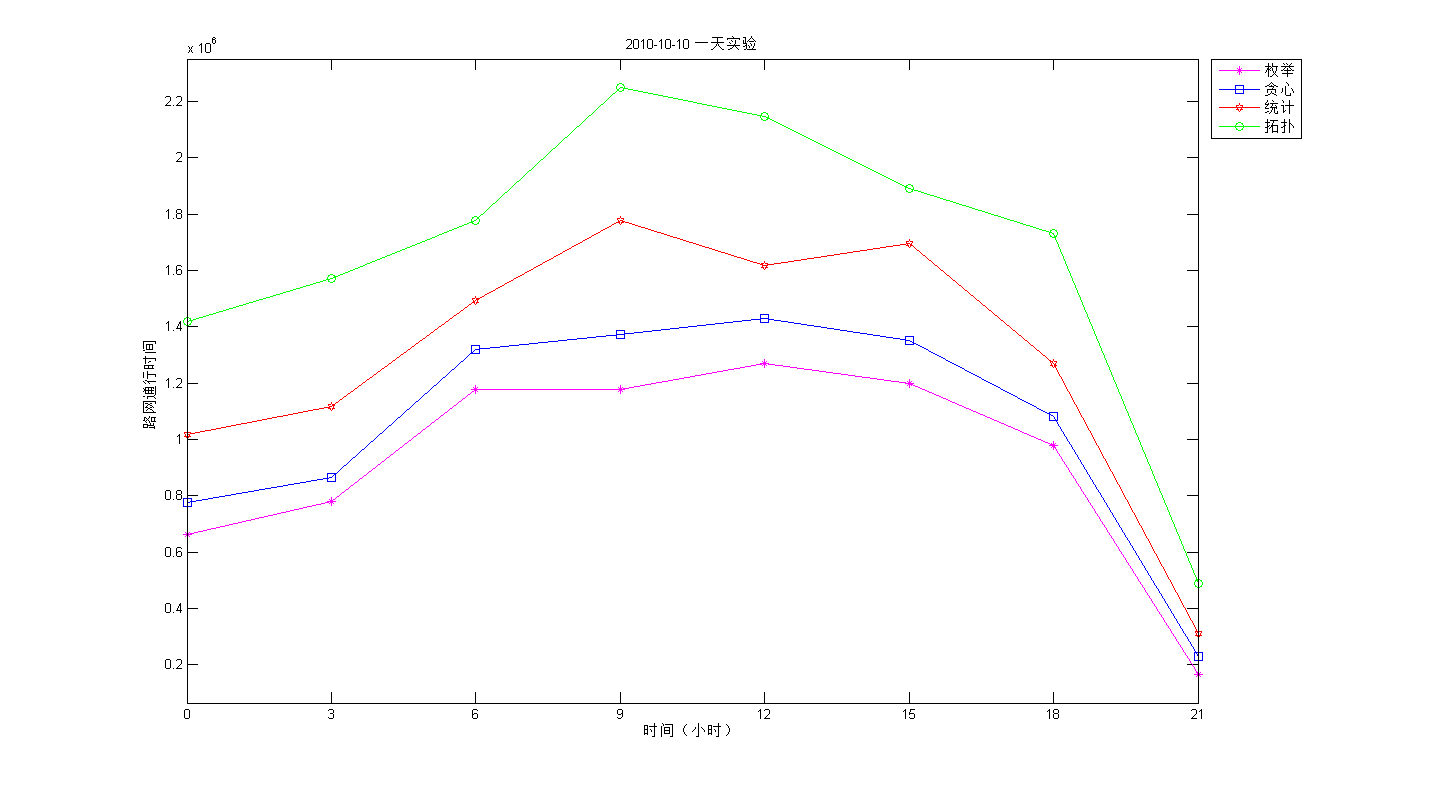
\includegraphics[width=3.0in]{picture/one_day_5}
					\caption{关键路段挖掘:以1h为区间}
					\label{fig1:a}
				\end{minipage}%
				\begin{minipage}{0.5\linewidth}
					\centering
					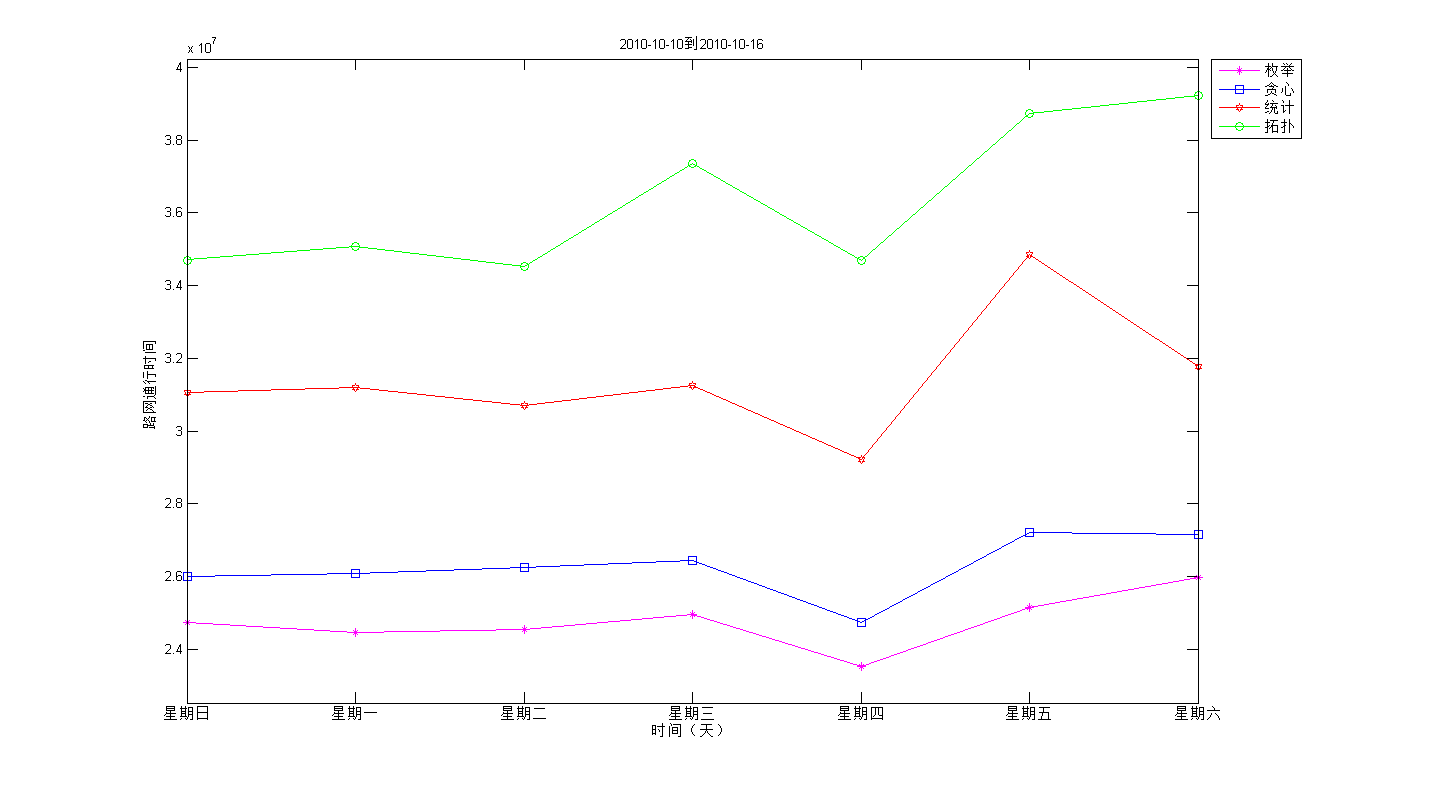
\includegraphics[width=3.0in]{picture/one_week_5}
					\caption{关键路段挖掘:以1d为区间}
					\label{fig1:b}
				\end{minipage}
				\end{figure}

				表\ref{tab:5}给出了不同方法求得的路网通行效率。表格中的数值是$L(\bm{y})$的绝对值(路网整体通行时间),可以看出贪心算法最接近最优解,而且误差在可接受范围内。

				\begin{table}[h]
				\centering
				\begin{tabular}{|c|c|c|c|c|}
				\hline
				\hline
				   &   枚举 &   贪心 &   统计 &   拓扑 \\
				\hline
				  一天 &  926030.06 & 1053575.26 & 1287439.55 & 1660243.55 \\
				\hline
				  一周 &  21674024.80 & 22989458.02 & 27510044.42 & 31790488.20 \\
				\hline
				\end{tabular}
				\caption{算法结果集}
				\label{tab:5}
				\end{table} 



				图\ref{fig2}给出了关键路段在路网中的分布图,图\ref{fig2}$(a)$是基于贪心算法求解的关键路段集合,图\ref{fig2}$(b)$是基于高速公路统计方法获得的路段集合。图\ref{fig2}$(c)$是基于枚举所得的最优解集,图\ref{fig2}$(d)$是基于路网拓扑结构选取的关键路段集合。对比图\ref{fig2}$(a)$和图\ref{fig2}$(b)$可以发现,直观上重要的点(承载流量较大的路段,事故多发路段等)并不一定在路网中属于关键路段集合,关键路段集合需要经过计算才能求出;直接枚举的路段集合与贪心算法求得的路段集合十分接近,平均有80\%以上的相似度,而统计和度中心性方法求得的关键路段和枚举方法差距较大。

						%插入图片
				%\10个收费站的情况下
				\begin{figure}
				%\begin{tabular}{cc}   
				\begin{minipage}{0.48\linewidth}
				  \centerline{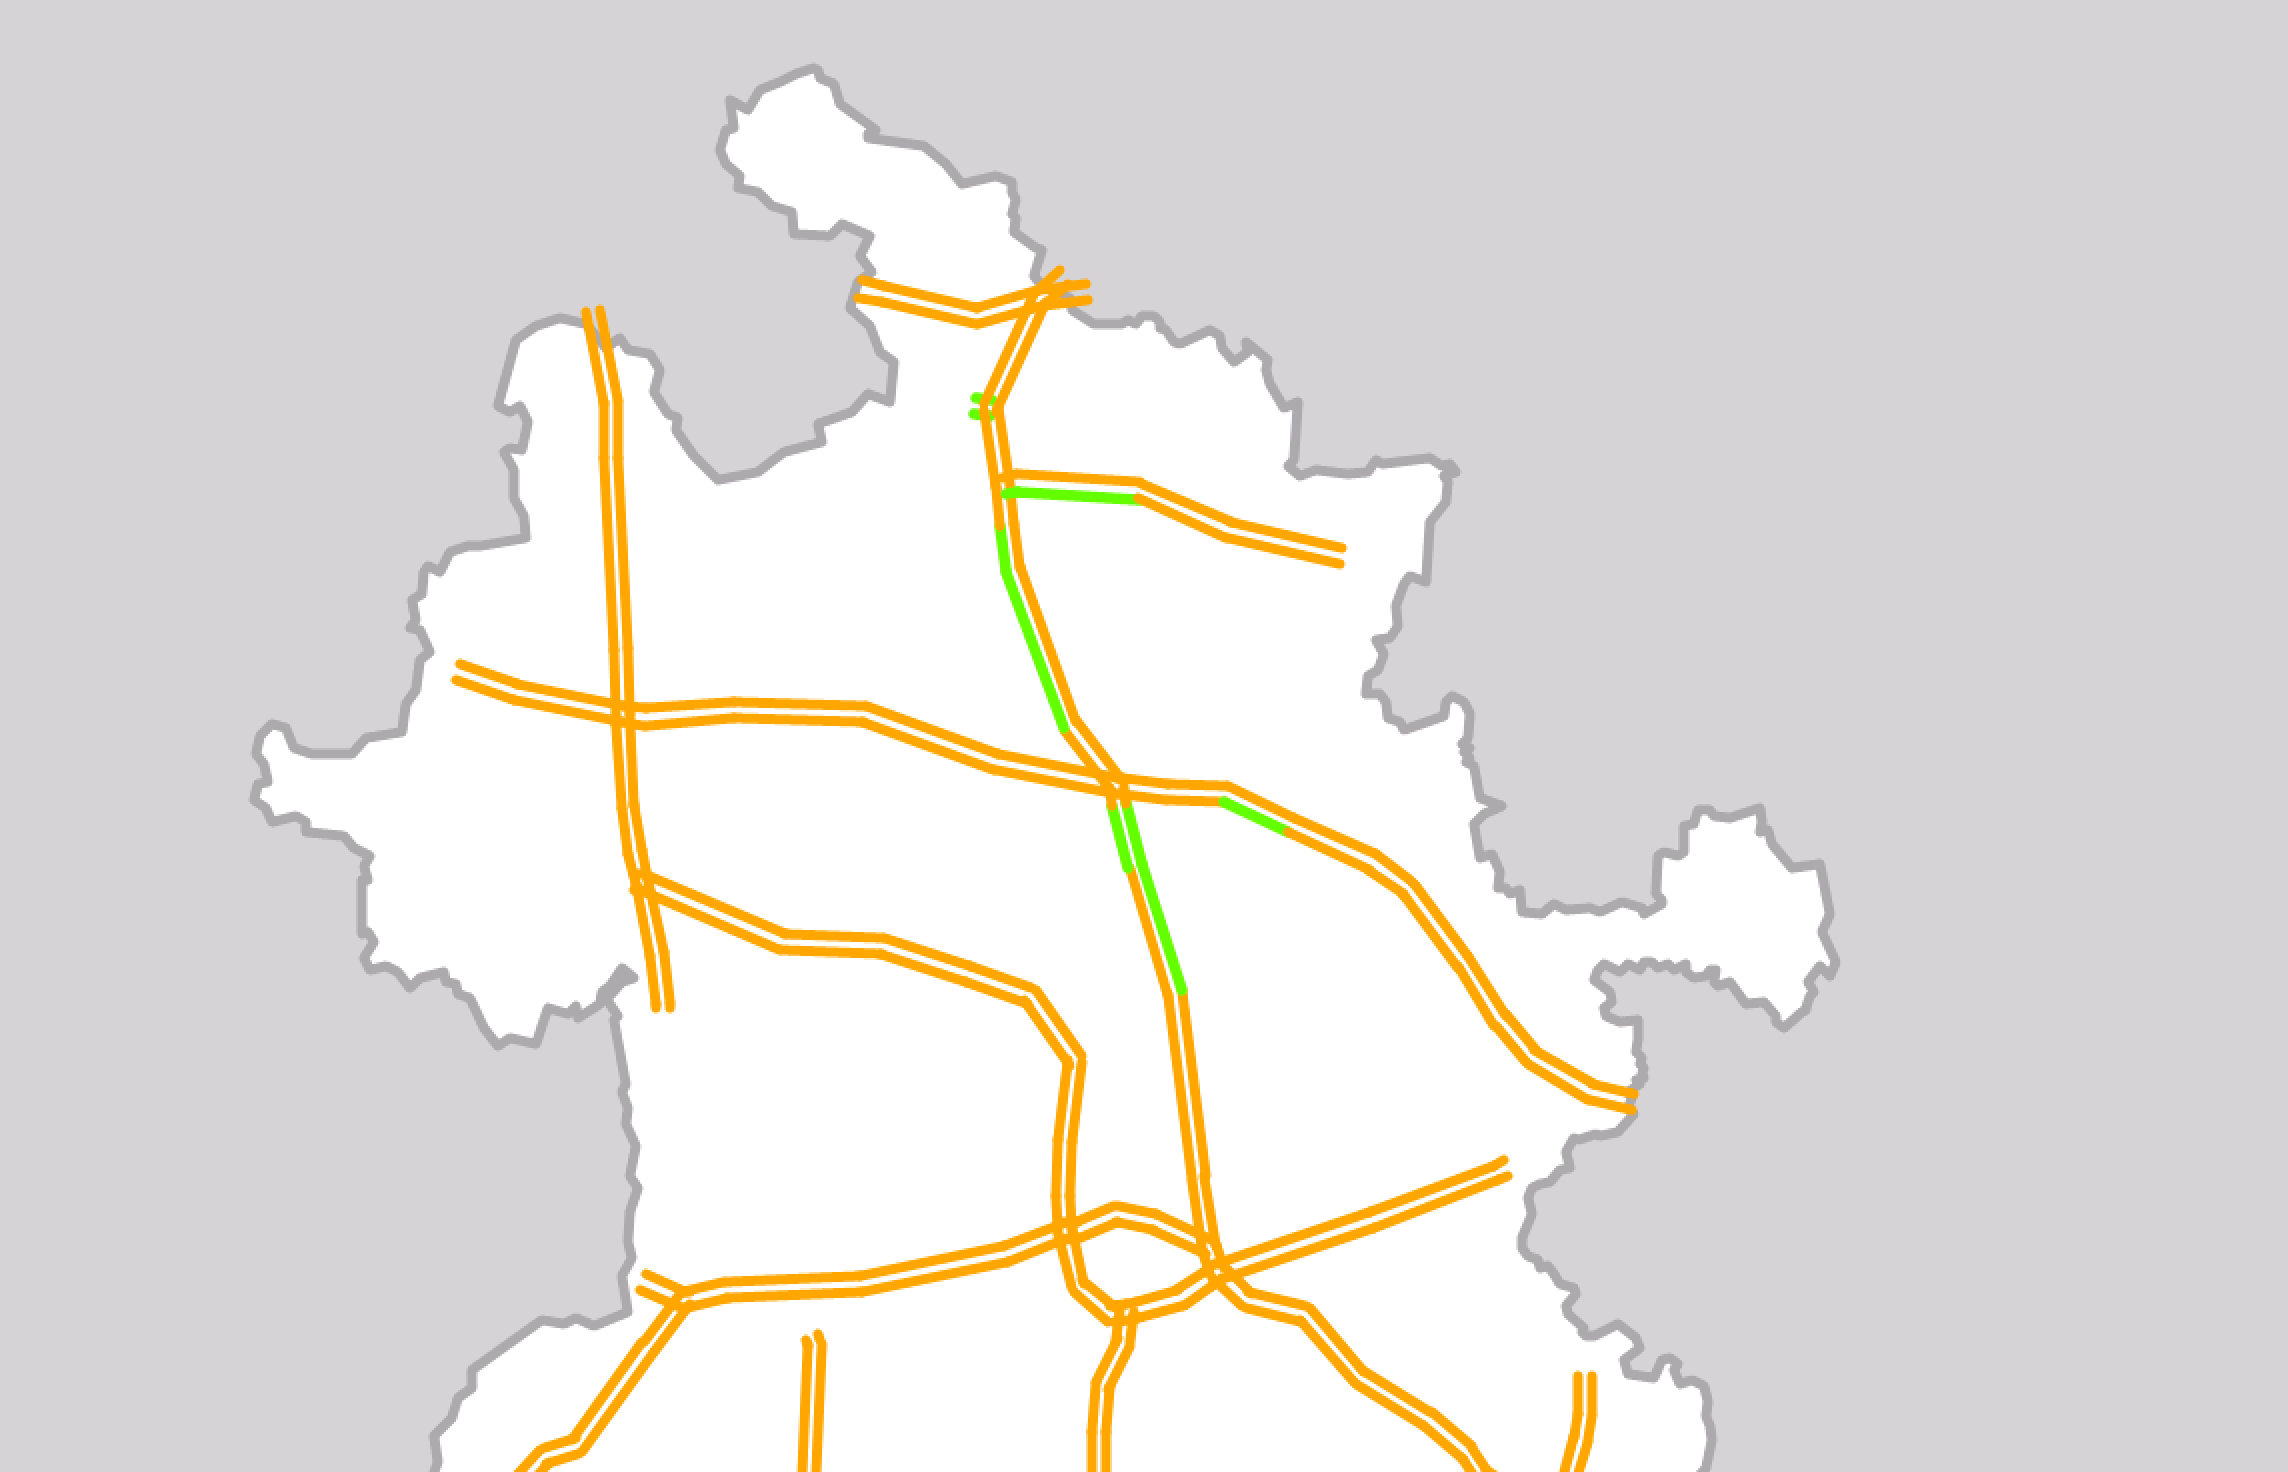
\includegraphics[width=3.0in]{picture/tanxin}}
				  \centerline{(a) 贪心算法关键路段}
				\end{minipage}
				\hfill
				\begin{minipage}{.48\linewidth}
				  \centerline{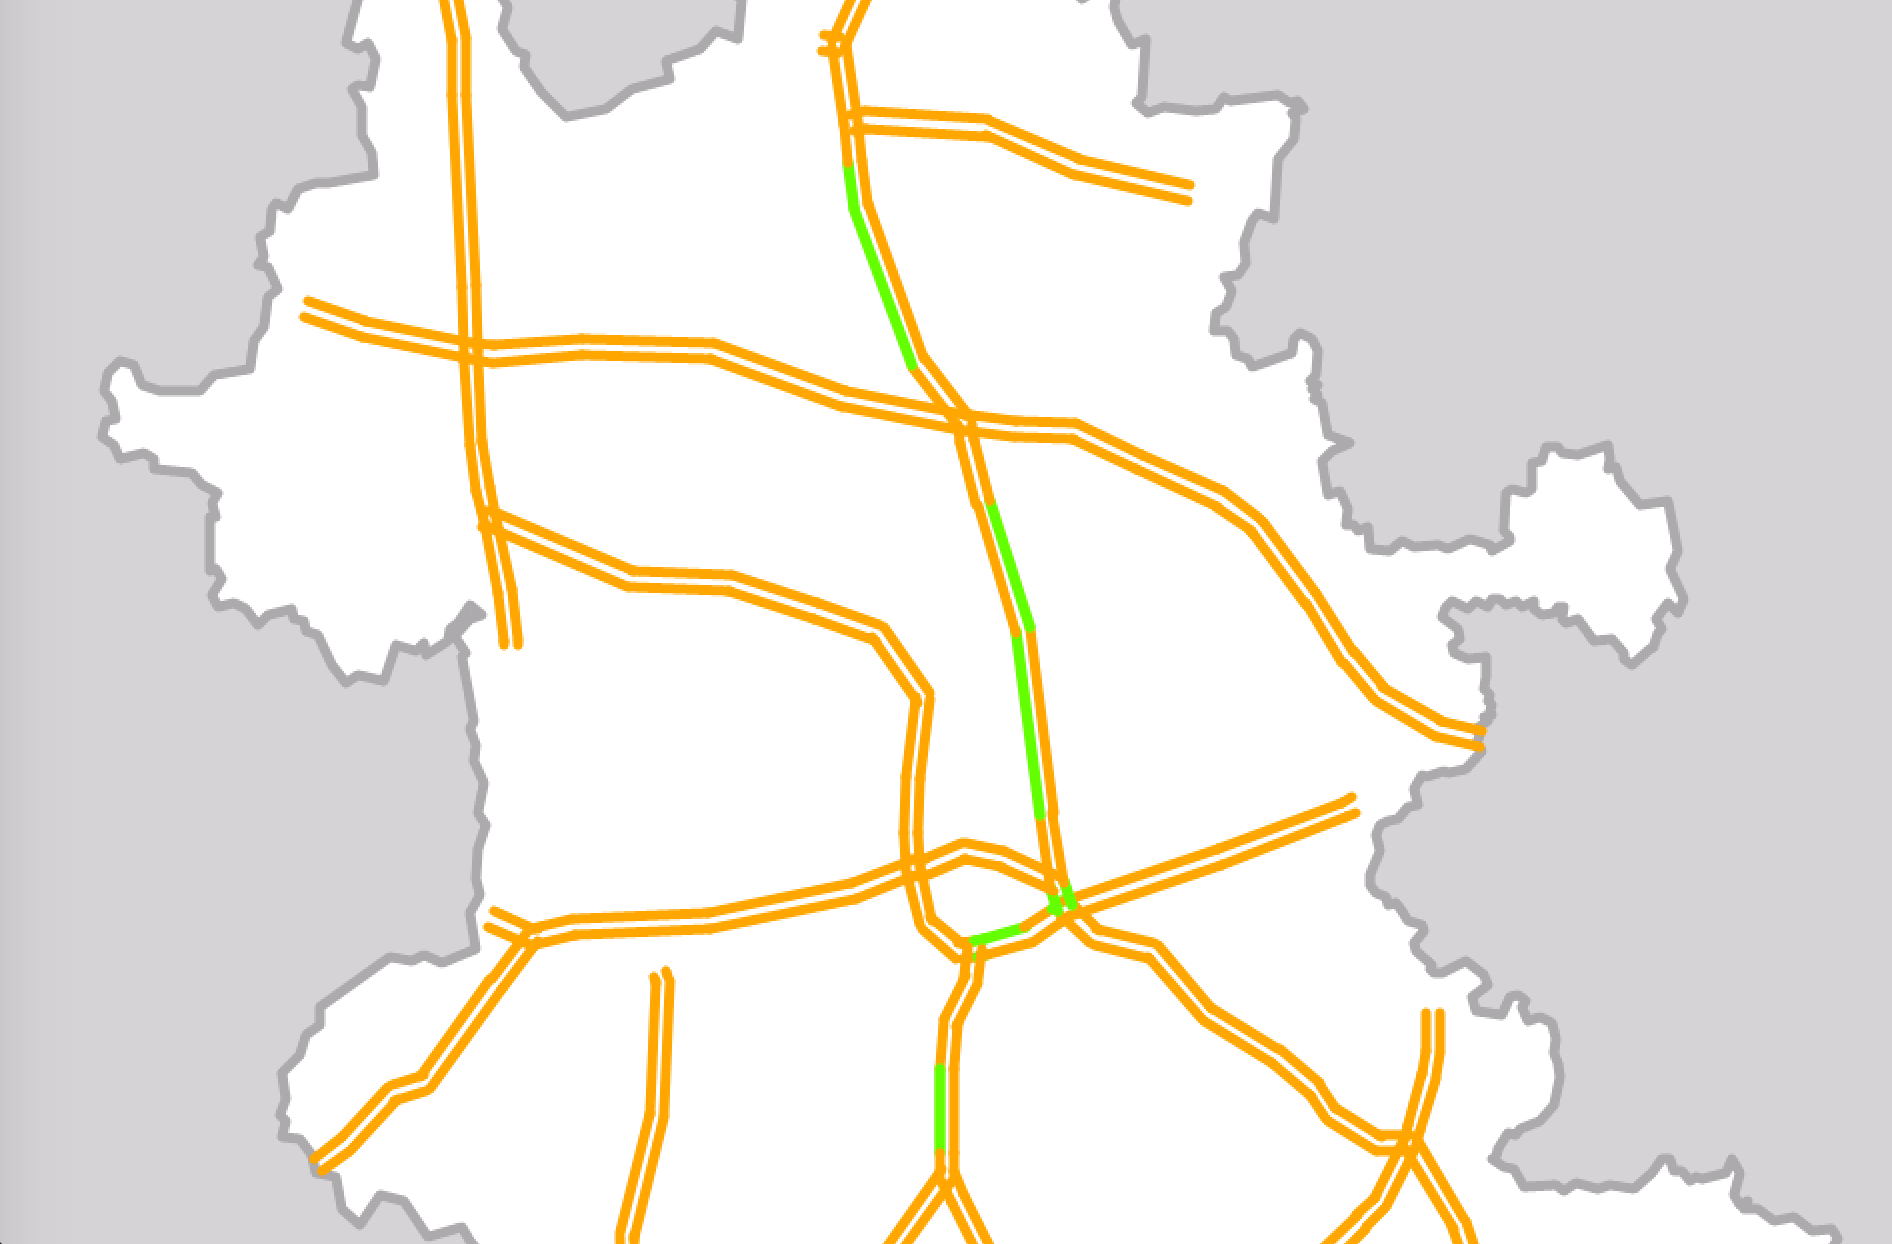
\includegraphics[width=3.0in]{picture/hotsection}}
				  \centerline{(b) 统计获得关键路段}
				\end{minipage}
				\vfill
				\begin{minipage}{0.48\linewidth}
				  \centerline{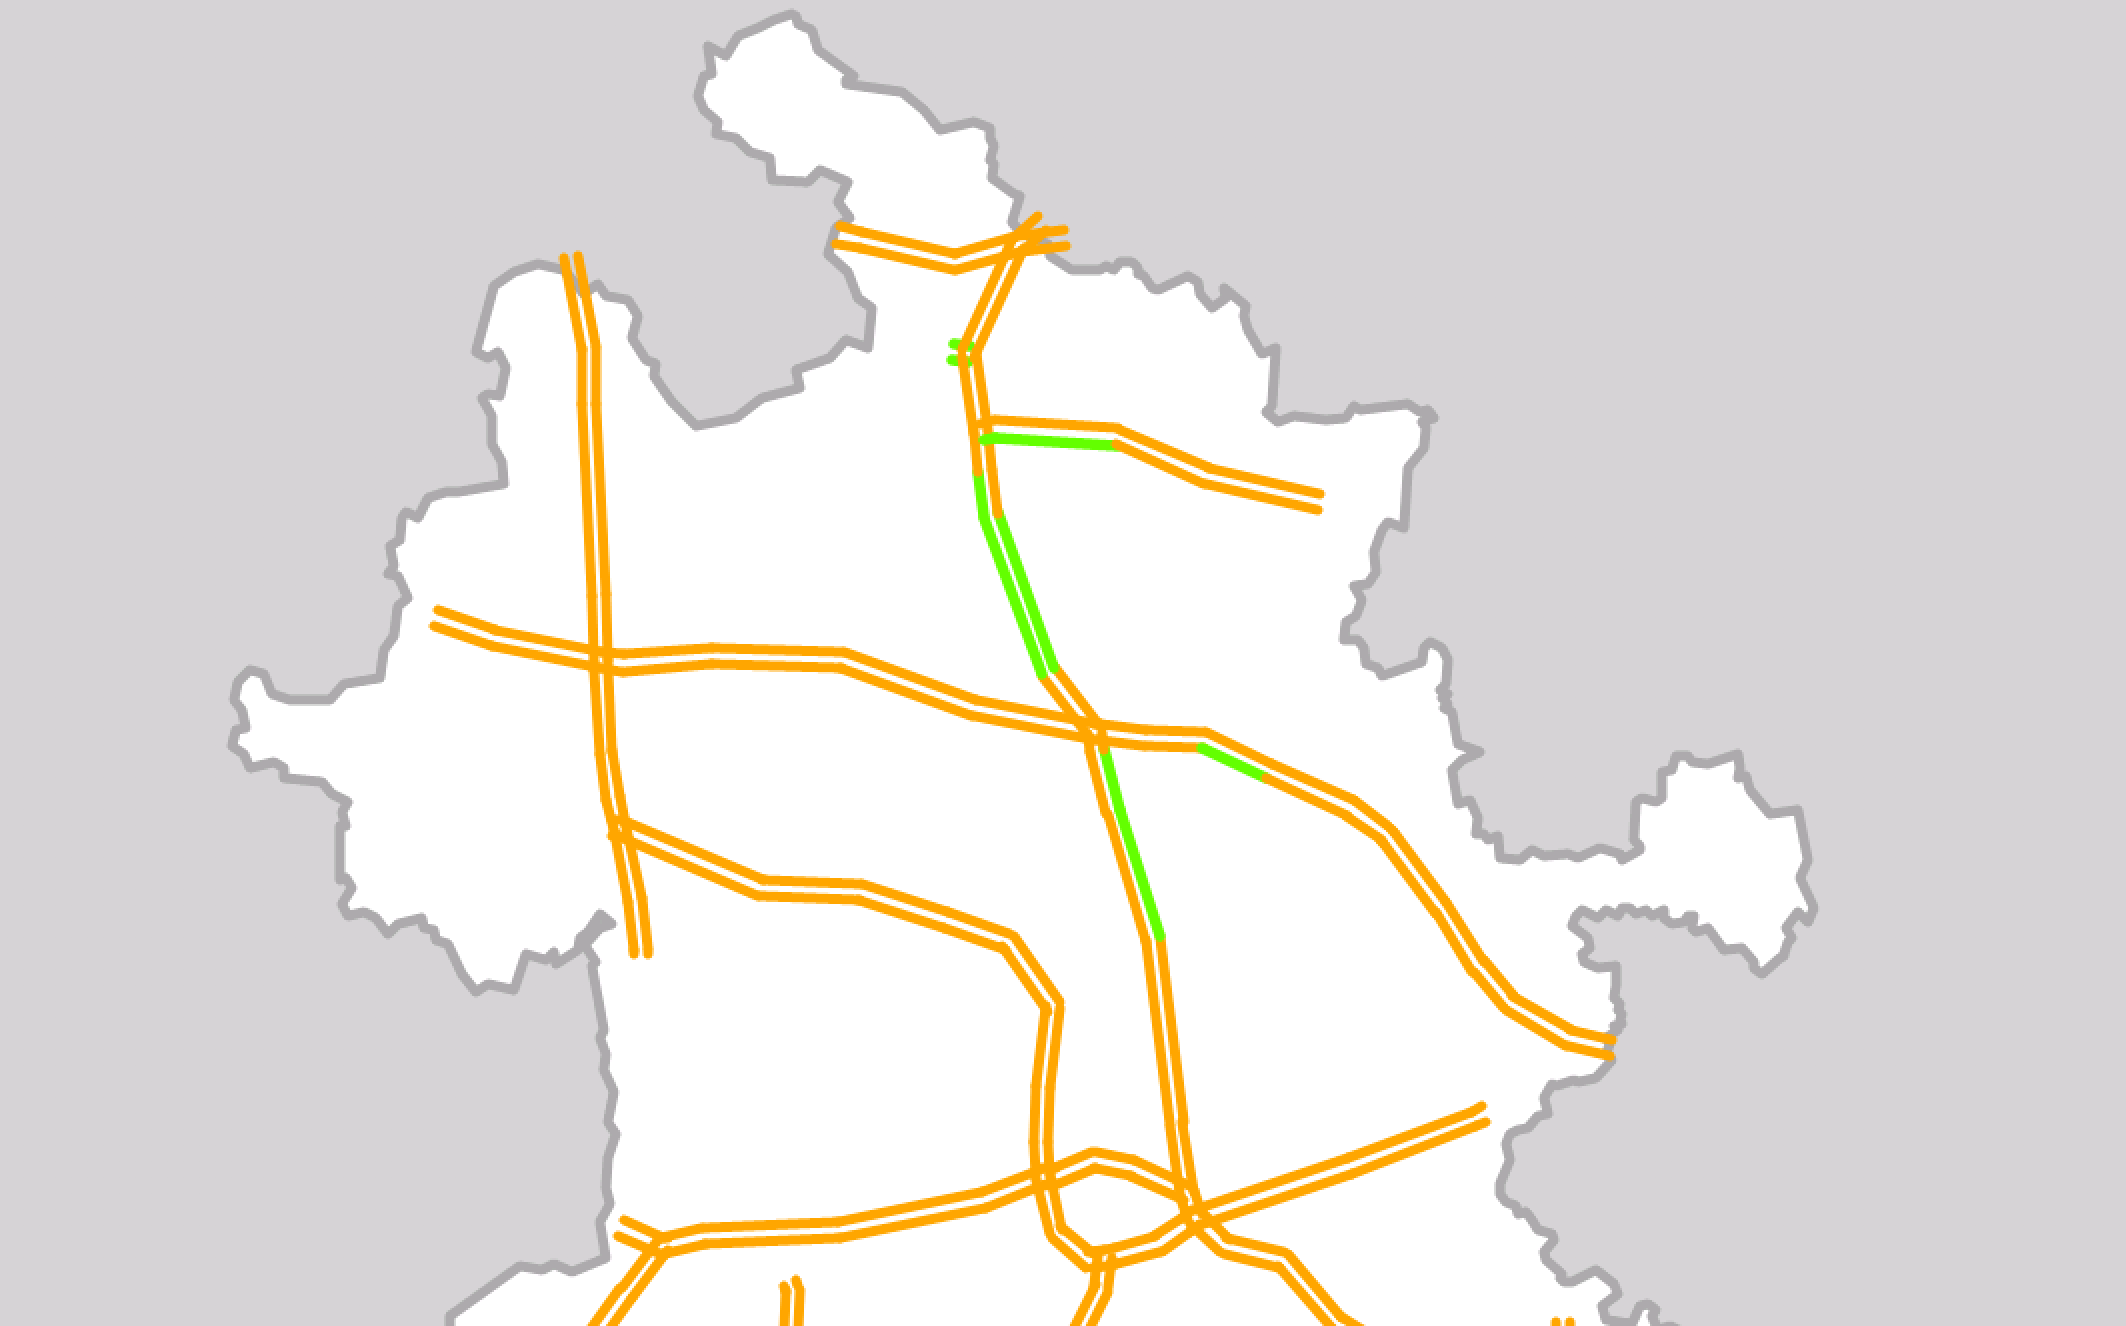
\includegraphics[width=3.0in]{picture/meiju}}
				  \centerline{(c) 枚举获得最优解}
				\end{minipage}
				\hfill
				\begin{minipage}{0.48\linewidth}
				  \centerline{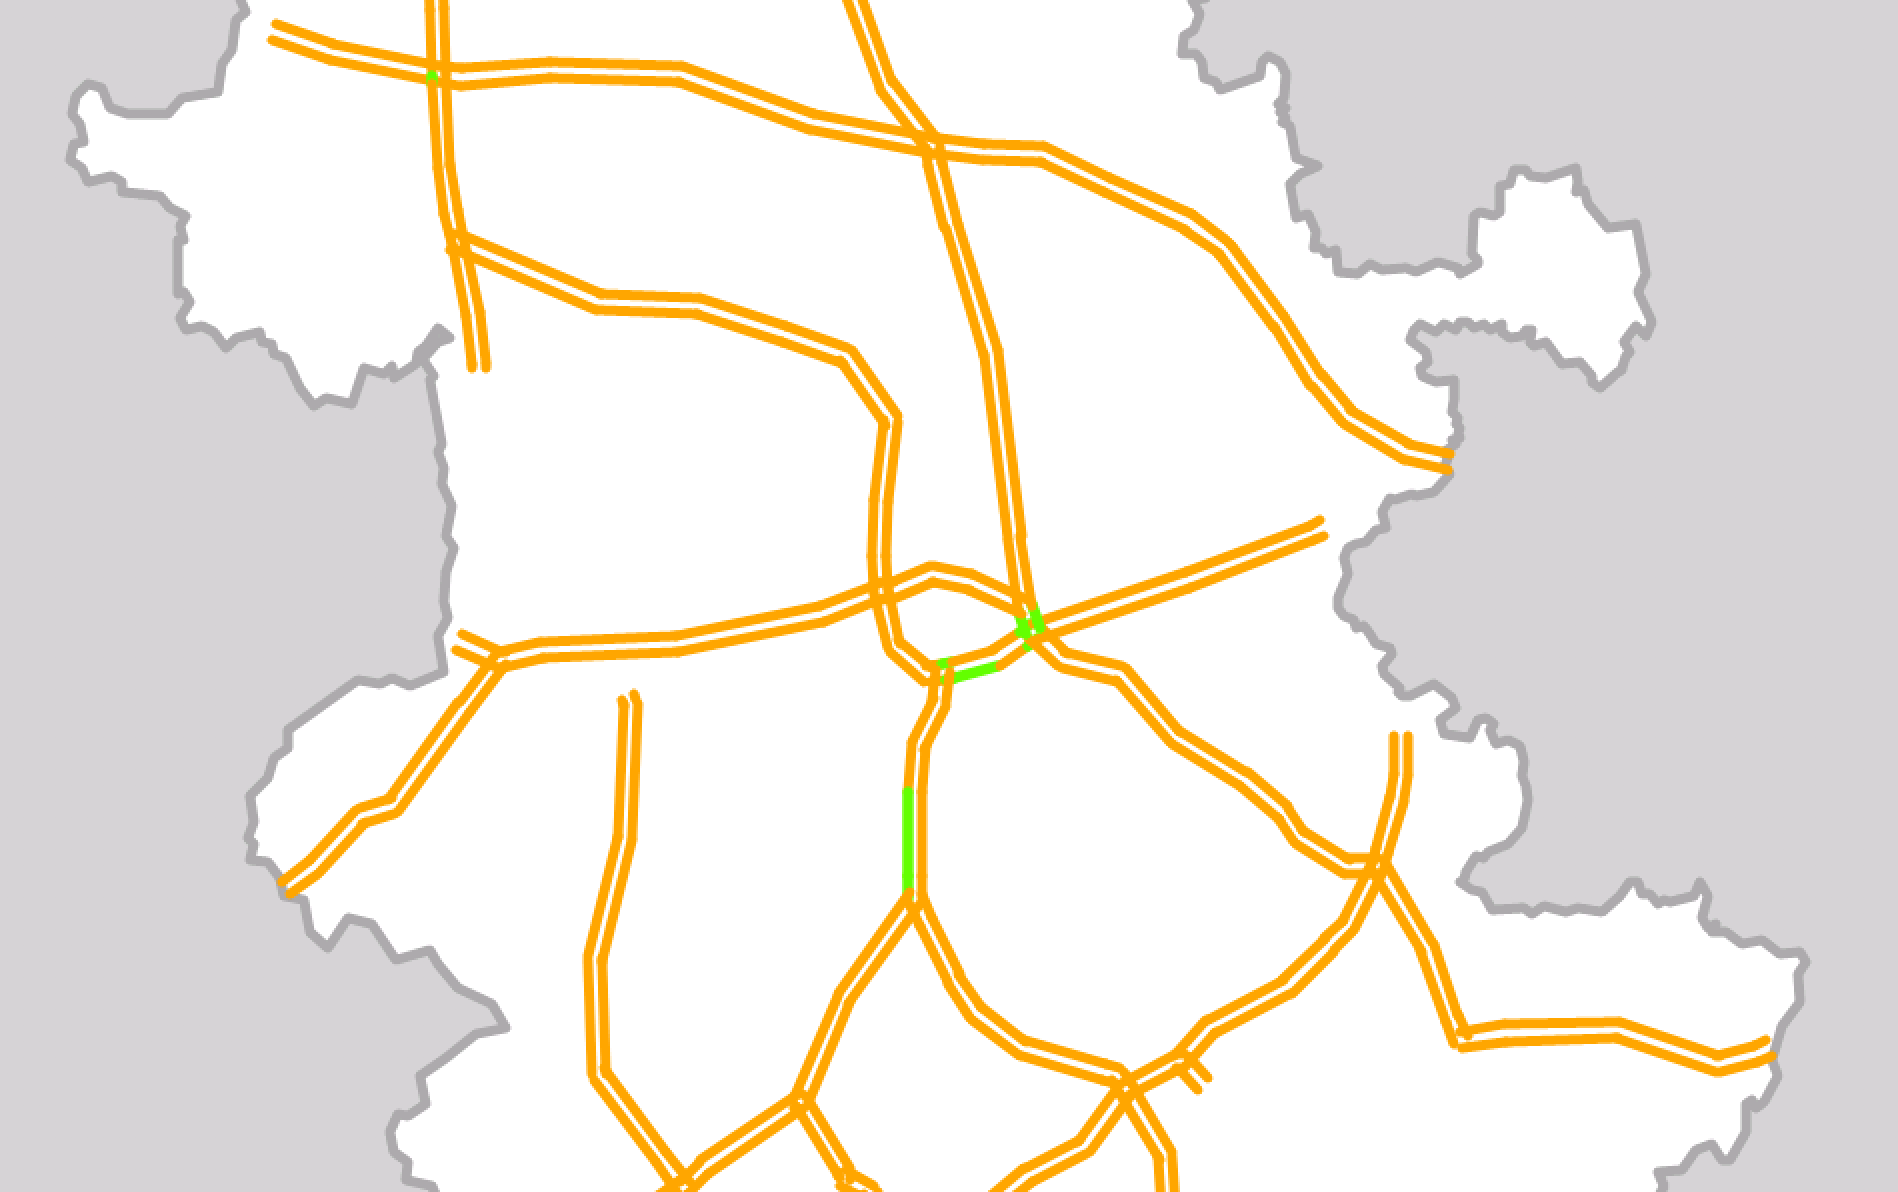
\includegraphics[width=3.0in]{picture/degree}}
				  \centerline{(d) 基于拓扑结构的关键路段}
				\end{minipage}
				%\end{tabular}
				\caption{不同方法求得的关键路段结果图}
				\label{fig2}
				\end{figure}

				在实验过程中,我们还发现当时间区间缩短到1h时,高速公路网络中的关键路段具有随着时间和流量变化而变化的特性。图\ref{duibi1}是凌晨3点时的高速公路关键路段集合,图\ref{duibi2}是早上九点时的高速公路关键路段集合。这一发现证明了高速公路的关键路段具有动态变化特性,即高速公路的关键路段不是一成不变的,而是会随着整个路网的流量的变化而变化。


				\begin{figure}[h]
				\begin{minipage}{0.5\linewidth}
					\centering
					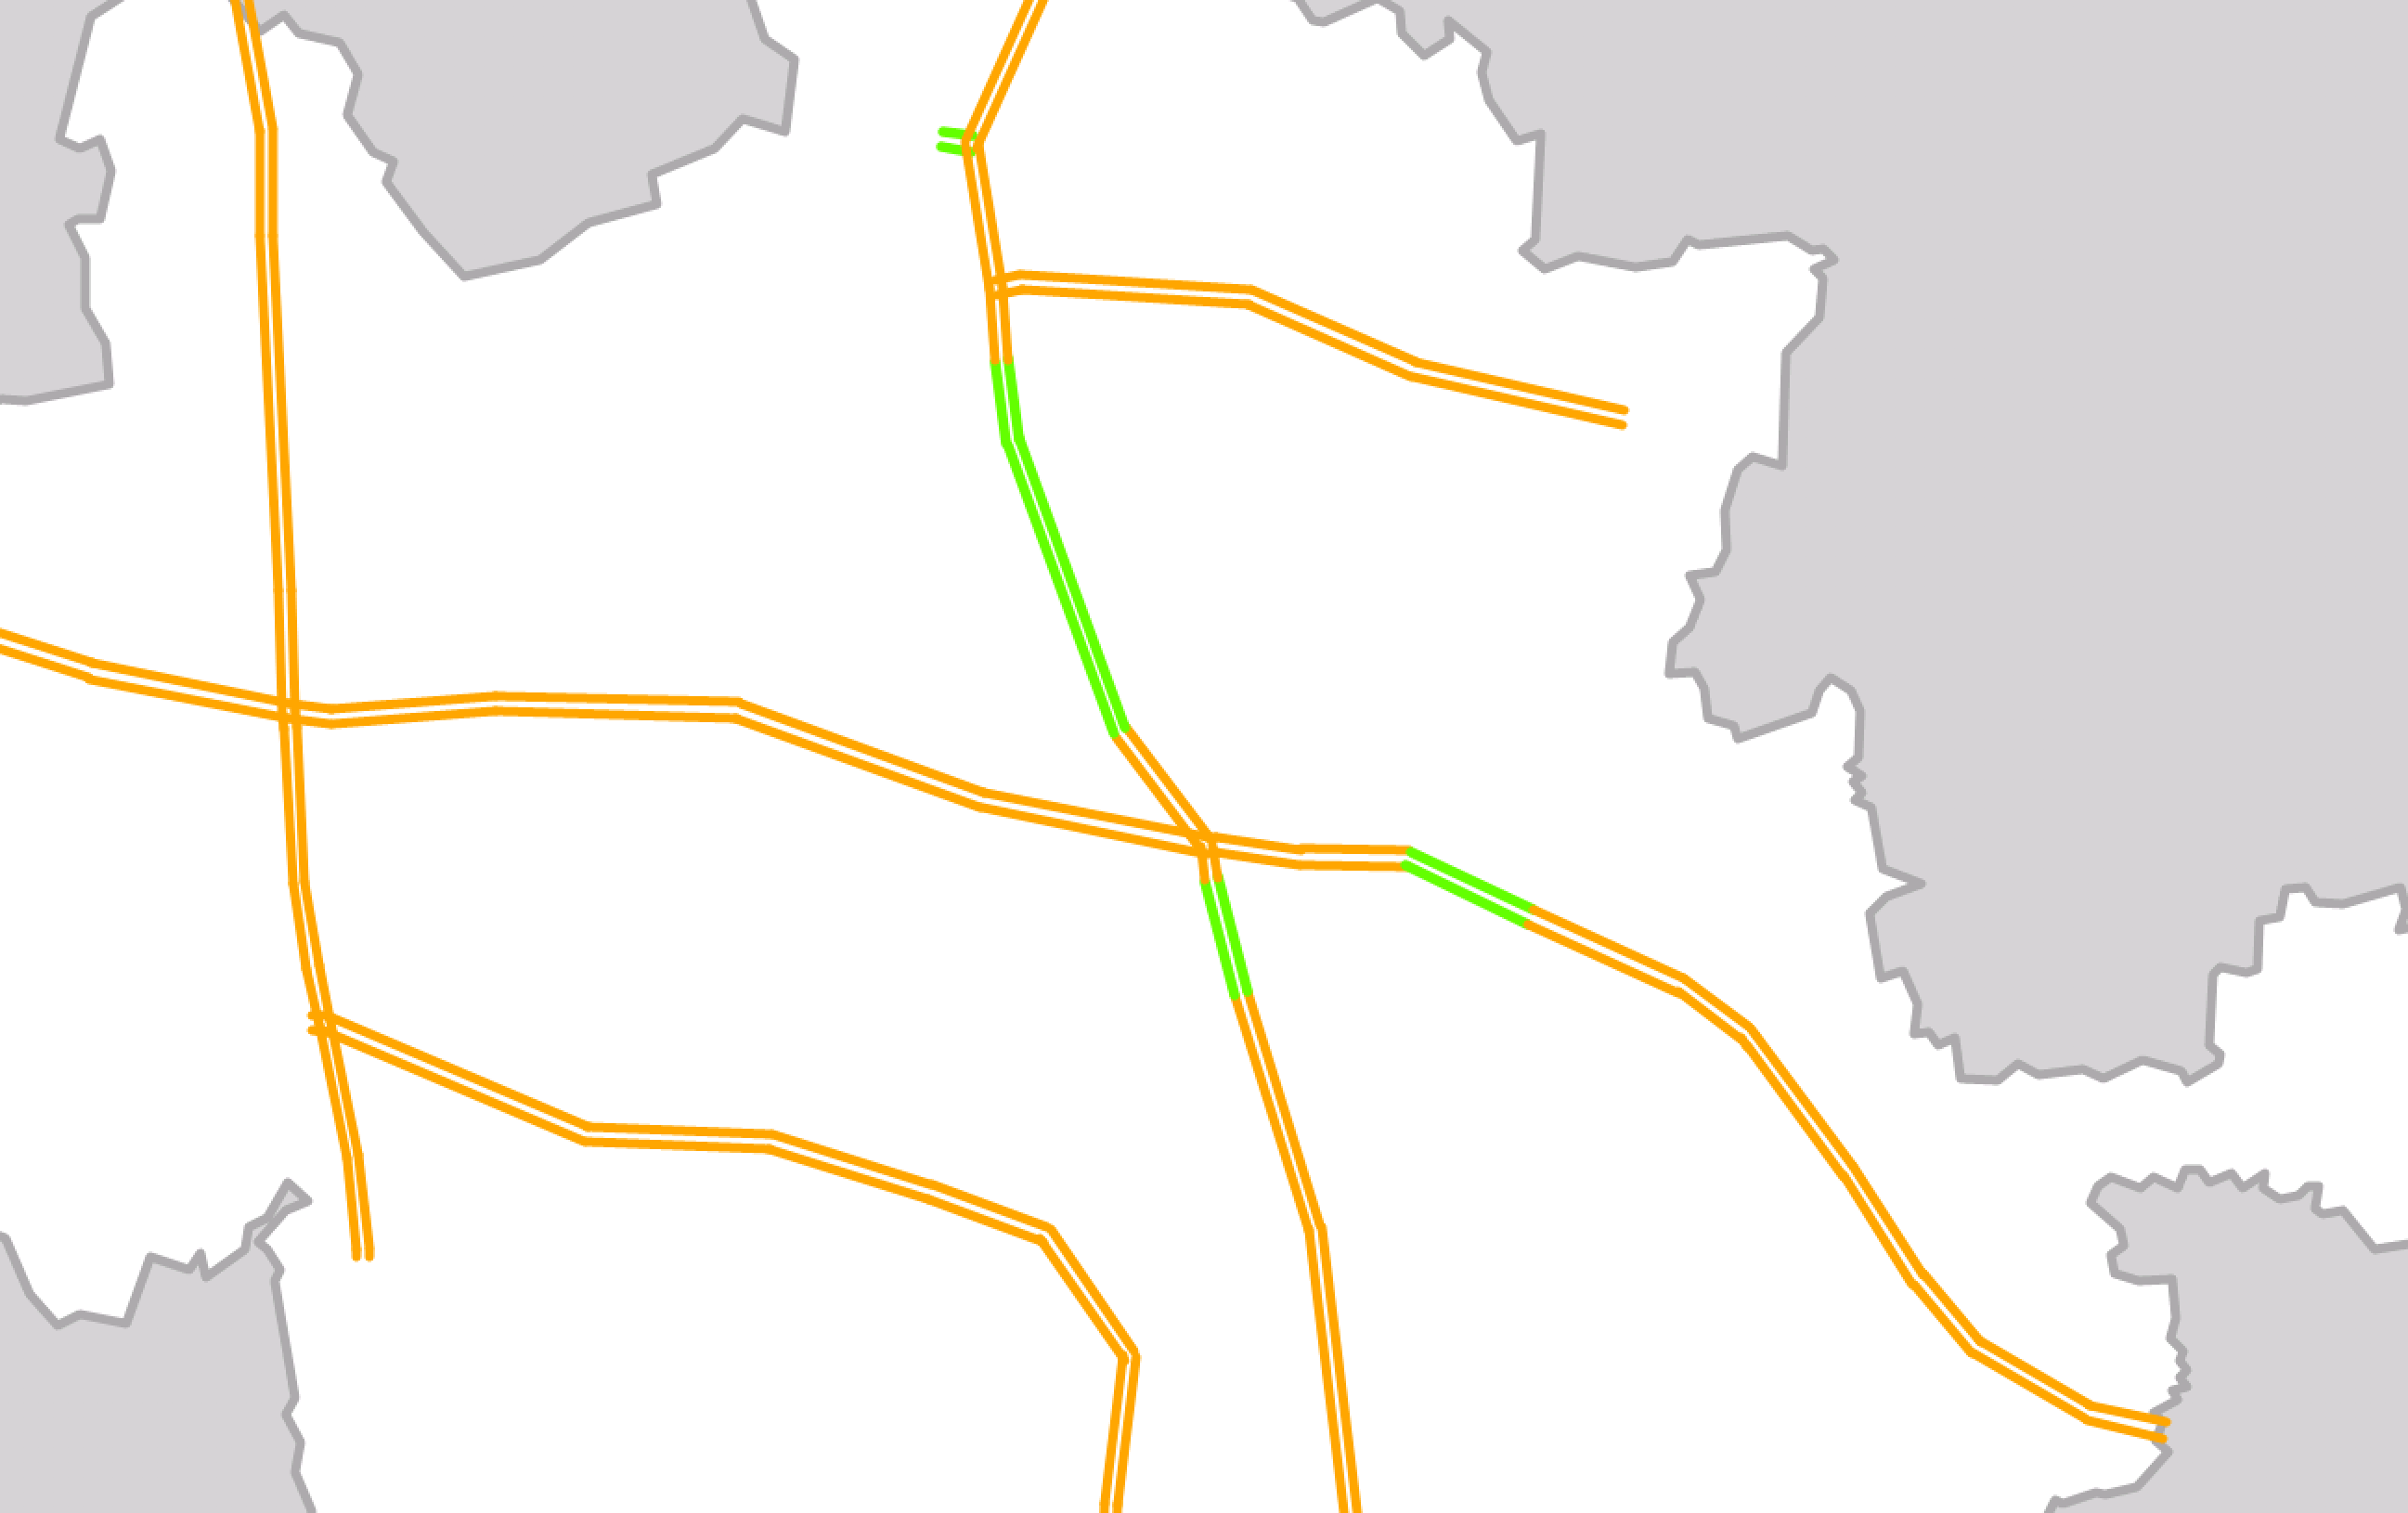
\includegraphics[width=3.0in]{picture/duibi1}
					\caption{关键路段挖掘:03:00}
					\label{duibi1}
				\end{minipage}%
				\begin{minipage}{0.5\linewidth}
					\centering
					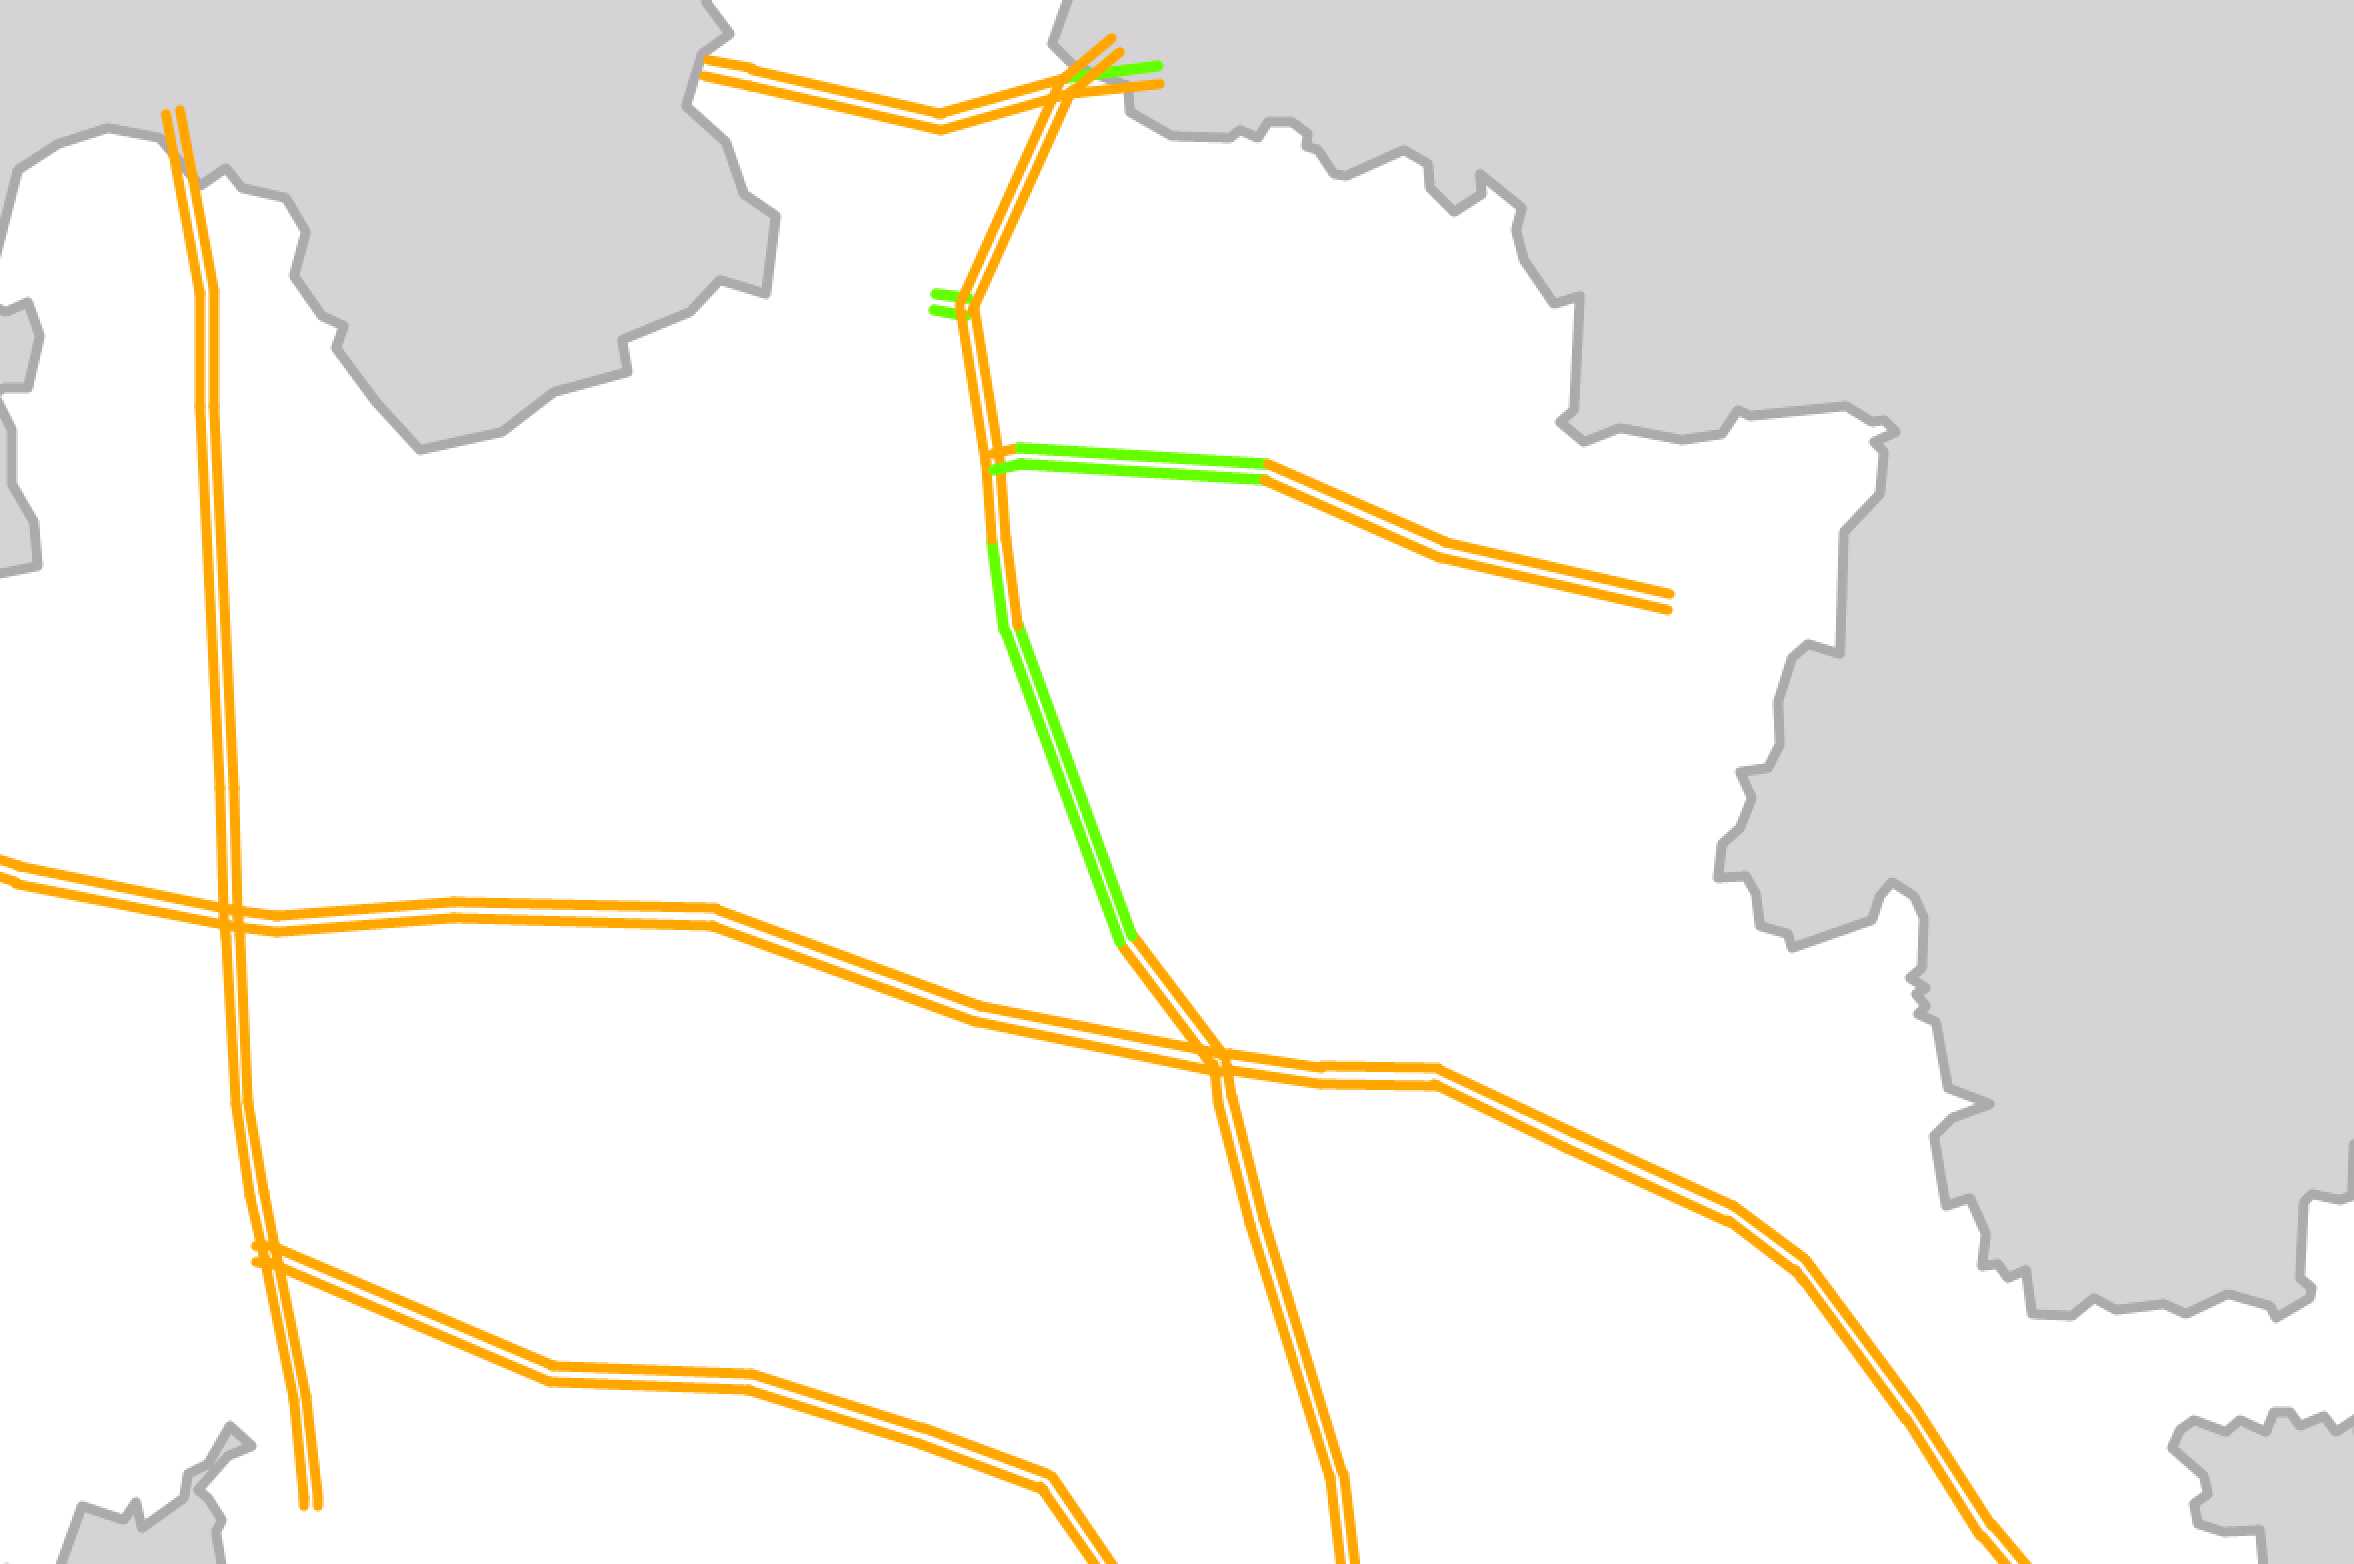
\includegraphics[width=3.0in]{picture/duibi2}
					\caption{关键路段挖掘:09:00}
					\label{duibi2}
				\end{minipage}
				\end{figure}

			\subsection{时间分析}
				基于暴力枚举方法的时间复杂度:$O({n^B}*{2^n})$

				基于贪心算法的时间复杂度:$O(n*B*{2^n})$

				基于统计路段重要性方法的时间复杂度:$O(n*\log (n))$

				基于路网拓扑结构方法的时间复杂度:$O(n*\log (n))$

				实验时间如表\ref{table1}所示,第一行代表实验的方法,第一列代表实验数据的范围,表格内的数值是实验的平均运行时间。

				\begin{table}[h]
				\centering
				\begin{tabular}{|c|c|c|c|c|}
				\hline
				\hline
				   &   枚举 &   贪心 &   统计 &   拓扑 \\
				\hline
				  一小时 &   1day &   30min &   1min &   1min \\
				\hline
				  一天 &   6day &   2h &   2min &   1min \\
				\hline
				  一周 &   7day &   3h &   5min &   1min \\
				\hline
				  一月 &   7day &   3h &   8min &   1min \\
				\hline
				\end{tabular}
				\caption{不同算法的运行时间}
				\label{table1}
				\end{table} 

				由表格可以看出,在以一个省为数据集的基础上,枚举方法已经处于一种较大的时间复杂度;贪心算法在一定程度上解决了算法过慢的情况,并且在精度上有一定的保证,可以应用于静态路网关键路段识别问题,但是对于动态实时应用仍旧不够;基于统计领域的路段重要性排序方法、基于路网拓扑结构的关键路段挖掘方法虽然在时间上效率较高,但是在精度上达不到要求。一周和一月的时间差距较小的原因是:对数据进行预处理,O-D相同的用户被归为一类。在时间区段增大到一定程度时,O-D类数量不再增加,算法运行时间增长较小。

		\section{本章小结}
			本章提出了一种面向高速公路网络的关键路段挖掘模型,同目前高速公路关键路段已有的挖掘方法相比,该方法的优势是结合高速公路的特性,考虑高速公路上的车流流量、路段事故率,从宏观角度提出一个整体的优化模型。针对上述模型,本章分析证明了模型的次模性,并给出基于贪心方法的关键路段挖掘方法。特别的,本文通过枚举方法,在较低的时间效率下计算高速公路中的最优解。结果表明该模型的贪心算法解可以很好地逼近真实解,并且在时间复杂度上有了规模性的优化,证明了贪心算法的可行性。然而,即使贪心算法可以在一定规模上优化整体的时间复杂度,并且可以在实际应用中运行良好,但是这是基于目前的研究目标是静态关键路段挖掘,同时高速公路也只有部分路段产生过断流等重大事故的情况下达成的。当任务环境更为复杂时(扩大到全国高速公路网络),当管理者需要更加迅速得到实时反馈的时候,上述方法受到算法计算规模的约束,无法达到预期的效果。下一章将针对高速公路的网络特性,给出相应的解决手段。





			
